\documentclass{article}
\usepackage[T1]{fontenc}
\usepackage{lmodern}
\usepackage{graphicx}
\usepackage{amsmath,amssymb}
\usepackage[a4paper,margin=2cm]{geometry}
\usepackage[absolute,overlay]{textpos}
\setlength{\TPHorizModule}{1mm}
\setlength{\TPVertModule}{1mm}
\usepackage[indonesian]{babel}
\usepackage{hyperref}
\setlength{\emergencystretch}{2em}
% unit: Halaman 45

\begin{document}

% === Halaman 45 (llm) ===

\vspace{207.31mm}

\begin{itemize}
    \item Al-Kindi menulis buku tentang seni memecahkan kode, buku yang berjudul 'Risalah fi Istikhraj al-Mu'amma (Manuscript for the Deciphering Cryptographic Messages)
    \item Al-Kindi menemukan frekuensi perulangan huruf di dalam Al-Quran. Teknik yang digunakan Al-Kindi kelak dinamakan \textbf{analisis frekuensi}.
    \item Yaitu teknik untuk memecahkan cipherteks berdasarkan frekuensi kemunculan karakter di dalam pesan
\end{itemize}

\vspace{20mm}

\textcolor{red}{Halaman pertama buku Al-Kindi, Manuscript for the Deciphering Cryptographic}

% deskripsi: Screenshot halaman pertama manuskrip bahasa Arab karya Al-Kindi tentang dekripsi pesan kriptografis.
% bbox normalisasi: [0.6160, 0.0670, 0.8030, 0.7650]
\begin{textblock*}{39.27mm}(129.36mm,19.90mm)
\noindent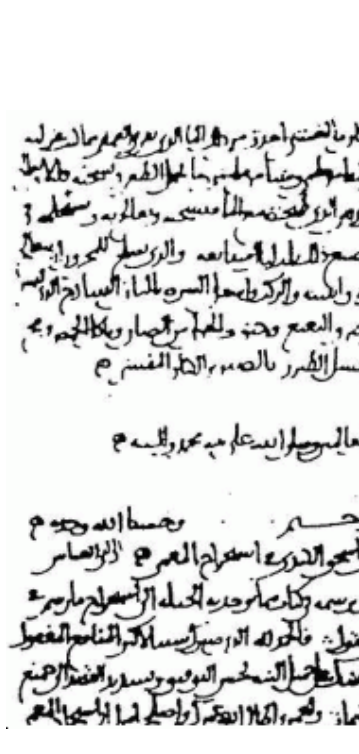
\includegraphics[width=39.27mm,height=207.31mm]{../../images/llm/page_045_img_01.png}%
\end{textblock*}

\end{document}
